\documentclass[main_conf.tex]{subfiles}

\begin{document}

Para medir la longitud se optará por colocar la hebra entre 2
rodillos, uno de ellos estará conectado a un disco encoder (ver
Fig. \ref{rodillo_con_disco}), este mismo será relativo y no
absoluto para minimizar costos al no utilizar más sensores. Este
encoder produce un código único digital para cada ángulo distinto
de rotación del eje conectado al rodillo (codigo Grey), cada
diente(estado ON/OFF) será detectado por un sensor fotoeléctrico
para encoder H2010, de tal manera que se cree un código binario
para cado uno de estos contactos.

\begin{figure}[!t]
  \centering
  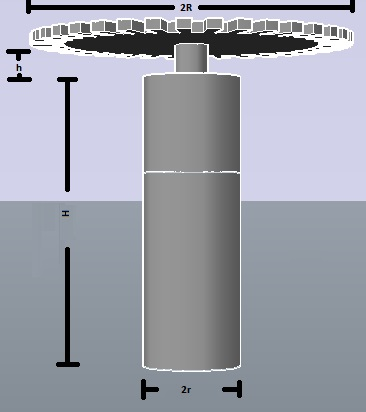
\includegraphics[width=2.5in]{../img/rodillo_con_disco.jpg}
  \caption{Rodillo con disco para encoder relativo}
  \label{rodillo_con_disco}
\end{figure}

\subsection{Cálculo del número de dientes y hendiduras}
\label{sec:estimador:dientes}
El sistema mide el número de ranuras desplazadas lo cual determinará
la longitud de la hebra fabricada. La longitud ($l$) está dada por
el ángulo que gira el rodillo ($\theta$) multiplicado por el radio
de este mismo ($r$) como se muestra en la ecuación
(\ref{eq:l_equal_theta_r}).

\begin{equation}
\label{eq:l_equal_theta_r}
l = \theta * r
\end{equation}

El ángulo de cada diente($\alpha$) es igual a una vuelta completa
entre el número de dientes($N$).

\begin{equation}
\label{eq:alpha_equ_2pi_N}
\alpha=\frac{2\pi}{N}
\end{equation}

Se elige un error($e$) máximo para la longitud.

\begin{equation}
e \leq 2 mm
\end{equation}

Este error es una variación del ángulo girado por el rodillo
multiplicado por el radio de este mismo.

\begin{equation}
\label{eq:delta_theta_r_leq_2mm}
\Delta  \theta *r \leq 2mm
\end{equation}

Por cuestiones de diseño se elige un diámetro de 3cm, para reducir
costo en acero, por lo que el radio es igual a:

\begin{equation}
\label{eq:r_equ_15mm}
r=15mm
\end{equation}

Reemplazando (\ref{eq:r_equ_15mm}) en
(\ref{eq:delta_theta_r_leq_2mm}) se halla el
valor de la variación del ángulo

\begin{equation}
\Delta  \theta\leq\frac{2}{15}
\end{equation}

Ésta variación del ángulo es multiplicada por el radio del disco
($R$) que da la longitud de un diente, por conveniencia se
elige un radio de disco igual a

\begin{equation}
R=5cm
\end{equation}

\begin{equation}
R*\Delta\theta\leq R*\frac{2}{15}
\end{equation}

\begin{equation}
\label{eq:max_L}
L\leq R*\frac{2}{15}
\end{equation}

La longitud del disco encoder en (\ref{eq:max_alpha}) se reemplaza
por el radio del disco y el ángulo del diente

\begin{equation}
R*\alpha\leq R*\frac{2}{15}
\end{equation}

\begin{equation}
\label{eq:max_alpha}
\alpha\leq \frac{2}{15}
\end{equation}

Reemplazando (\ref{eq:max_alpha}) en (\ref{eq:alpha_equ_2pi_N}) se
obtiene

\begin{equation}
\frac{2\pi}{N}\leq \frac{2}{15}
\end{equation}

\begin{equation}
\label{eq:15pi_leq_N}
15\pi \leq N
\end{equation}

La ecuación (\ref{eq:15pi_leq_N}) determina el mínimo número de
dientes que debería tener el disco para que el error máximo sea
2mm. Para reducir el error aún más, se elige $N=72$.

\subsection{Cálculo del error de la medición}

Se deduce de (\ref{eq:delta_theta_r_leq_2mm}) el error de la
longitud dada en la siguiente fórmula

\begin{equation}
\label{eq:e_equ_alpha_r}
e = \alpha * r
\end{equation}

Reemplazando (\ref{eq:alpha_equ_2pi_N}) en (\ref{eq:e_equ_alpha_r}) se
obtiene

\begin{equation}
e = \frac{2\pi}{N} * r
\end{equation}

Reemplazando con el nuevo valor de $N$

\begin{equation}
e = 1.3mm
\end{equation}

Para implementar el sistema con el sensor H2010 es necesario saber
cual es número de ranuras desplazadas($k$), que es igual a
la longitud desplazada del rodillo entre la longitud de cada diente

\begin{equation}
k = \frac{R * \theta}{R * \alpha}
  = \frac{\theta}{\alpha}
\end{equation}

\begin{equation}
k = \frac{\theta}{2\pi}*N
\end{equation}

\subsection{Dimensionamiento del rodillo con disco}
Se dimensionarán 4 medidas que se muestran en la Fig.
\ref{rodillo_con_disco}. Estas son:

\begin{itemize}
\item $H$: altura del tronco del rodillo
\item $h$: altura del eje entre el rodillo y el disco
\item $R$: radio del disco
\item $r$: radio del rodillo
\end{itemize}

Empezando por $H$, podemos ver que las es la altura del tronco
del rodillo con disco y debe ser más grande que la altura de la
HM más grande a fabricar por lo que se decide asignar

$$ H = 90 mm $$

La siguiente variable es $h$, la altura del eje que une el
rodillo con el disco encoder. Se elige un valor que proteja
al disco ante cualquier desvío de la HM.

$$ h = 10 mm $$

Dado los cálculos hechos en \ref{sec:estimador:dientes} se
determina los siguientes valores:

$$ R = 50 mm $$
$$ r = 15 mm $$

\end{document}
